% !TeX encoding=utf8
% !TeX spellcheck = en-US

\chapter{Methods}



\section{Data}

\begin{figure}[H]
  \centering
  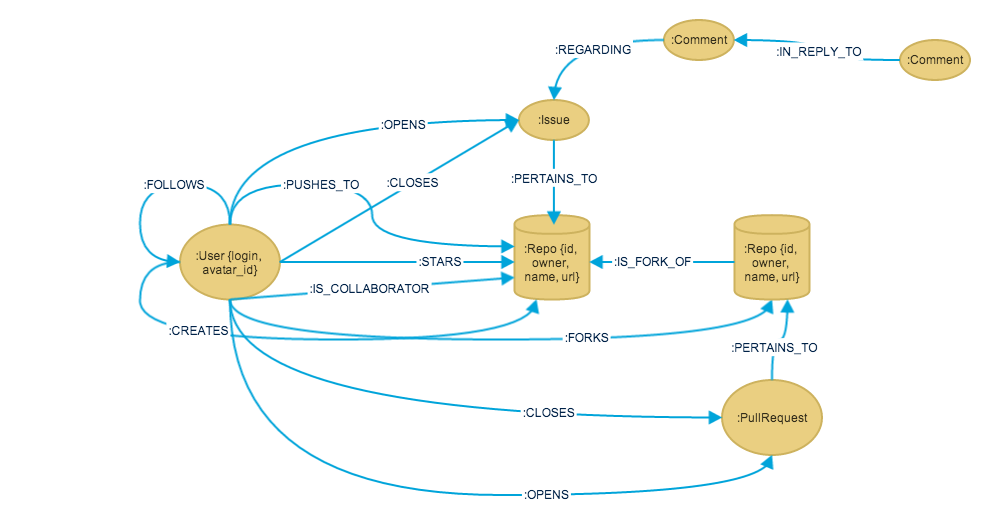
\includegraphics[width=0.75\textwidth]{images/githubdatamodel.png}
  \caption[GitHub graph data model]{GitHub data model as a labeled property graph.}
  \label{fig:figures:1}
\end{figure}


Data was collected from GitHub Archive\cite{githubarchive}, a service that maintains an archive of all public events emitted by the GitHub API\cite{github:Online}. These include events such as creation of new repositories, pushes to repositories, repository stars, and user follows. Data was collected for the time period April 1st, 2013 - April 1st, 2014. For the purposes of this project, only \textit{FOLLOWS} events were considered. This resulted in a total of 539893 users and 919489 follows. In terms of a graph, that equates to 539893 nodes and 919489 vertices between nodes.

\begin{figure}[ht]
\vskip 0.2in
\begin{center}
\centerline{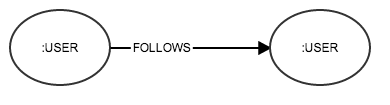
\includegraphics[width=0.3\columnwidth]{images/user_user.png}}
\caption[User-User data model]{The GitHub follow graph is a simple graph with User nodes and Follows edges.}
\label{fig:figures:4}
\end{center}
\vskip -0.2in
\end{figure} 

A graph data model is used to represent this data as the data is highly connected: it is describing entities (users and repositories) and their interactions (stars, follows, pushes, etc). Figure \ref{screenshot-data} shows an example of a subgraph of user and repository nodes and the interactions among those entities, modeled as a graph.

\subsection{Data munging}
The data from GitHubArchive is available in streaming JSON format and includes all public events generated from the GitHub event API \cite{github:Online} for a given time period. The one year of data collected for this project resulted in several thousand JSON files, each several megabytes in size resulting in a raw dataset of several hundred gigabytes. As this project is only concerned with the user-user {\textit FOLLOWS} relationship, the data is parsed using a Python script to filter for only those {\textit FOLLOWS} events. For further efficiency, the data is reduced to an anonymized edgelist format:
\begin{verbatim}
    1	2
    3	4
    5	6
    7	8
    9	10
    11	12
    11	13
    14	15
    16	17
    18	19
    ...
\end{verbatim}
This allows for the dataset to be anonymized using only arbitrary user ids and stored as compactly as possible. In the above example (and in the context of a directed graph) the first column corresponds to the source node and the second column the destination node. So the sample above represents: user 1 follows user 2, user 3 follows user 4, ...

This edgelist file is then used to populate a Neo4j graph database instance, using only the minimal information necessary to implement our link prediction system. 

\begin{table}[t]
\caption{Dataset descriptive statistics}
\label{results}
\vskip 0.15in
\begin{center}
\begin{small}
\begin{sc}
\begin{tabular}{rrccr}
\hline
Nodes (users) & 539893  \\
Edges (:FOLLOWS relationships) & 919489 \\
Mean degree & 3.4 \\
Standard deviation of degree & 30.3 \\
\hline
\end{tabular}
\end{sc}
\end{small}
\end{center}
\vskip -0.1in
\end{table}


\begin{figure}[ht]
\vskip 0.2in
\begin{center}
\centerline{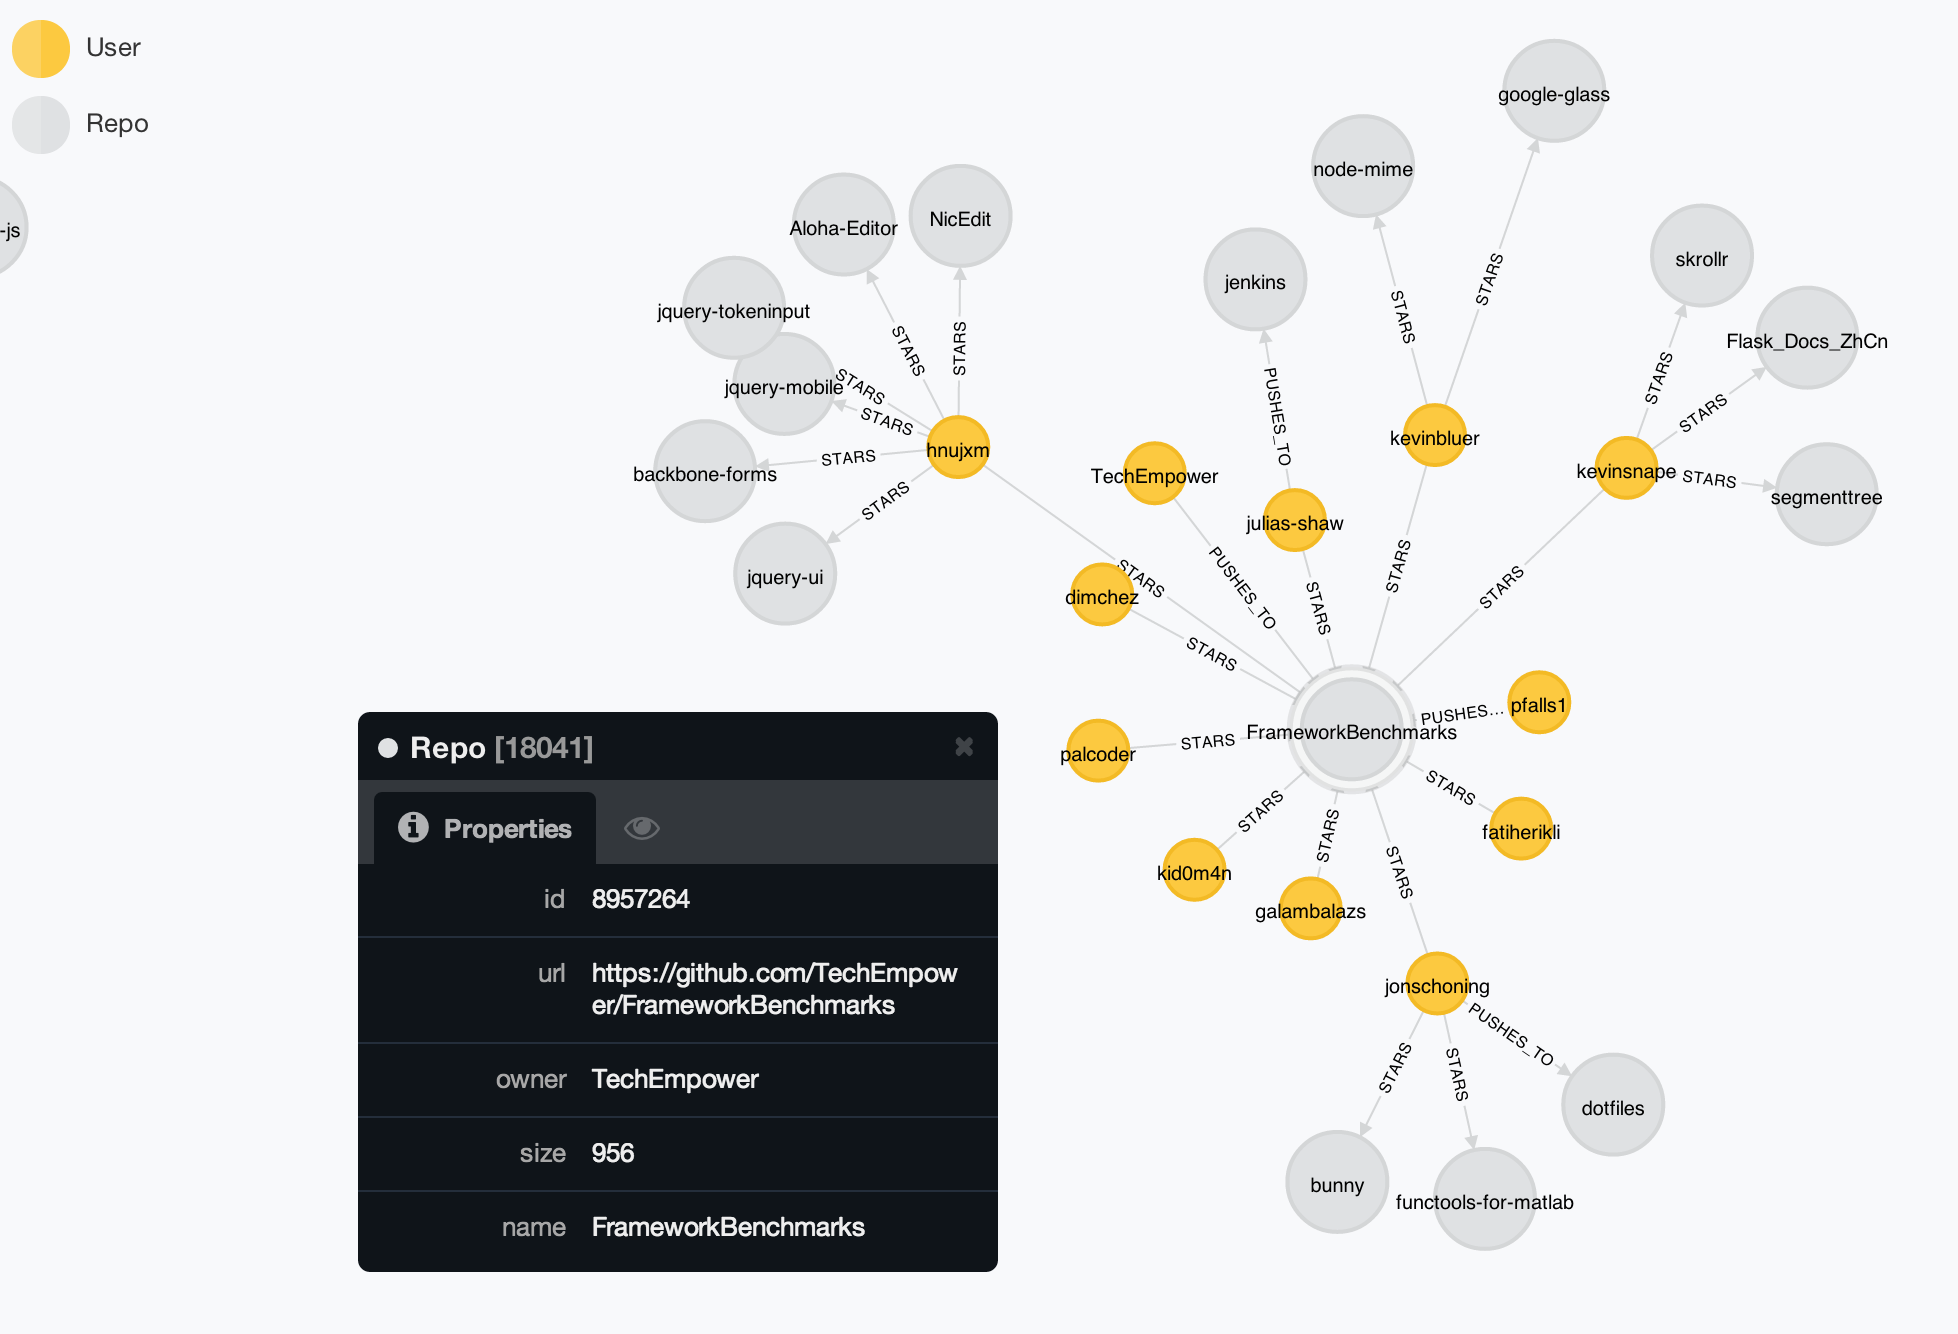
\includegraphics[width=\columnwidth]{images/neo_screenshot.png}}
\caption{GitHub data model as a property graph. Screenshot from Neo4j graph database interface.}
\label{screenshot-data}
\end{center}
\vskip -0.2in
\end{figure} 

\section{Algorithms}

\subsection{Sample Graph}
Draw a sample graph. Based on this graph we will examine specifically how to calculate CF using jaccard (and maybe some other similarity metrics from the table in Schall)

\subsection{Collaborative Filtering}
Collaborative filtering is a method of generating recommendations based on the homophily principle: users who are similar are likely to be interested in similar items. It is implemented by finding similar users, allowing each similar user to "vote" for recommendations and suggested items with the highest score. This is similar to the kNN algorithm used for classification.\cite{cf}
\subsubsection{Similarity Metrics}
The Jaccard index is used to identify similar users. For two users, $a$ and $b$, let $A$ and $B$ denote the sets of all users being followed by $a$ and $b$, respectively. The Jaccard index is therefore as defined in Equation \ref{jaccard}.
\begin{equation}
\label{jaccard}
J(A,B) = \frac{|A \cap B|}{|A \cup B|}
\end{equation}

In this context, Jaccard is defined as the intersection of the users followed by $a$ and $b$ divided by the union of the users followed by $a$ and $b$. This results in a number between 0 and 1, indicating the strength of similarity between users $a$ and $b$.
 
%\begin{algorithm}[tb]
%
%  \caption{Collaborative Filtering Recommendation}
%   \label{alg:cf}
%\begin{algorithmic}
%   \STATE {\bfseries Input:} Graph $G(V,E)$, vertex $v$, int k
%   
%   \FOR{$i=1$ {\bfseries to} $m-1$}
%   \IF{$x_i > x_{i+1}$} 
%   \STATE Swap $x_i$ and $x_{i+1}$
%   \STATE $noChange = false$
%   \ENDIF
%   \ENDFOR
%  
%\end{algorithmic}
%\end{algorithm}

\subsection{Triadic Closeness}

\section{Implementation}

\subsection{Graph Data Model}
The labeled property graph

\subsection{Graph Traversal Pattern}
What is the graph traversal pattern? The graph traversal pattern allows us to design algorithms where the answer to our question is a traversal through the graph. 

\subsection{}
\begin{figure}[ht]
\vskip 0.2in
\begin{center}
\centerline{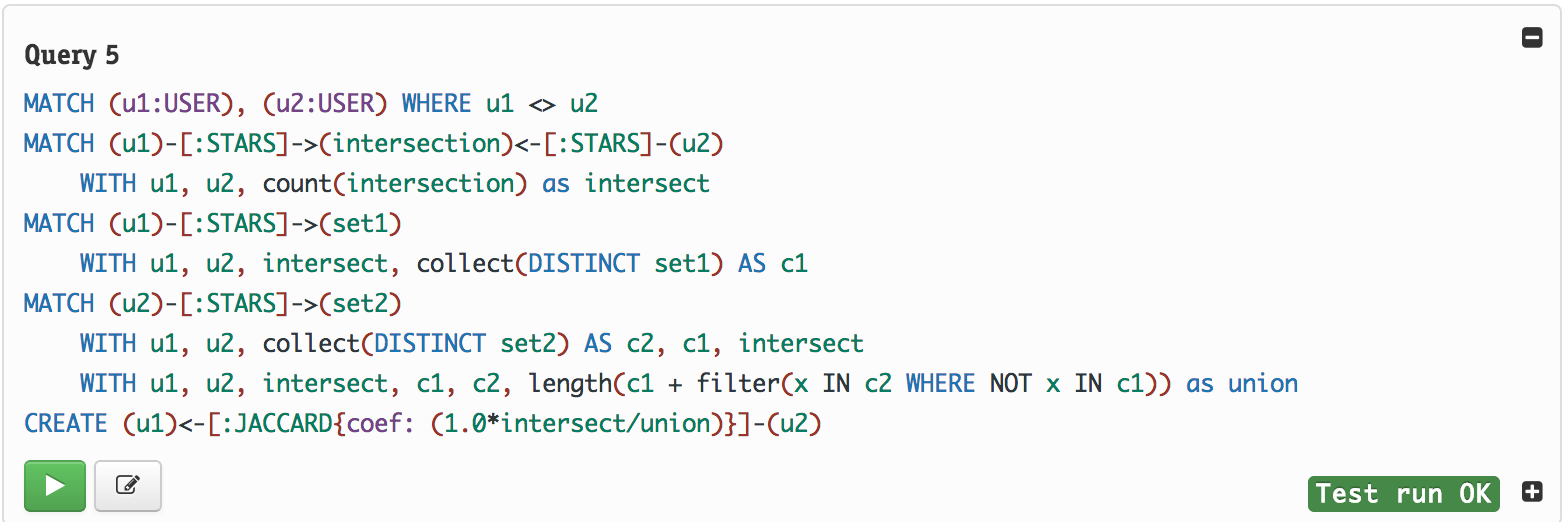
\includegraphics[width=\columnwidth]{images/jaccard.png}}
\caption{Example of Neo4j Cypher query language used to calculate Jaccard metric for pairs of users.}
\label{icml-historical}
\end{center}
\vskip -0.2in
\end{figure} 
The system is developed using Java and makes use of the Neo4j graph database. The Cypher query language is used to query the graph database and for defining graph traversals for processing. The program is configurable and implements k-fold cross validation.

\subsection{Steps}
The following describes implementation of the system at a high level. For each validation fold:

\begin{itemize}
\item Select $p$ users at random
\item For each user $u$ in $p$:
	\begin{itemize}
	\item Remove one $FOLLOWS$ edge $f$ for this user at random
	\item Find $k$ nearest neighbors using Jaccard index (ensure removed edge is not used for this calculation)
	\item Calculate $n$ followed users with greatest overlap (the most commonly followed users among the $k$ nearest neighbors)
	\item Return set of $n$ users, these are the recommended users
	\item Is $f$ in $n$? If yes, this run is counted as a valid prediction.
	\end{itemize}
\item Report summary accuracy metrics for this fold
\end{itemize}


